\documentclass[../../main.tex]{subfiles}
\begin{document}
\section{Applicazioni alle derivate}
\subsection{Studio di funzioni}
Definiamo i punti di massimo e di minimo relativo.\\
Sia $f(x)$ definita in un intervallo $[a, b]$.\\
\begin{center}[h]
    \begin{figure}
        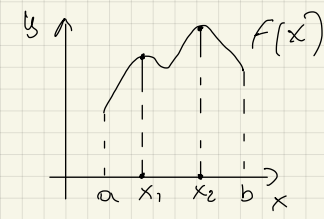
\includegraphics{studiofunzioni.png}
    \end{figure}
\end{center}

\begin{itemize}
    \item $x_1\in[a, b]$ è un punto di \textbf{massimo relativo} per $f$ nell'intervallo $[a, b]$ se il valore $f(x_1)$ è più grande dei valori
          $f(x)$ per ogni $x$ nell'intervallo $[a, b]$ vicino ad $x_1$. Più precisamente se $\exists \delta > 0$
          tale che $f(x_1) \geq f(x)$ per ogni $x\in[a, b]$ tale che $|x-x_1|<\delta$.
    \item $x_2$ è un punto di \textbf{massimo assoluto} per $f$ se $f(x_2)\geq f(x)$ per ogni $x\in[a, b]$.
\end{itemize}
Analogamente per i punti di minimo con $\leq$ al posto di $\geq$.\\
\textbf{Osservazione:} Tutti i punti di massimo o minimo interni all'intervallo $[a, b]$ (cioè $\in(a, b)$) hanno retta tangente orizzontale in quel punto cioè del tipo:
\[
    y = q
\]
(Non vale per gli estremi per gli estremi dell'intervallo $x=a,b$, ma con $x_0\in(a, b)$).\\
Ricordando la retta tangente al grafico di una funzione in $x_0$
\[
    y = f(x_0) + f'(x_0)(x-x_0)
\]
questa retta è orizzontale $\iff f'(x_0) = 0$.\\

\subsection{Teorema di Fermat}
Sia $f$ una funzione definita in $[a, b]$ e sia $x_0$ un punto di massimo o di minimo relativo interno ad $[a, b]$.
Se $f$ è derivabile in $x_0$, alora risulta:
\[
    f'(x_0) = 0
\]
\textbf{Dimostrazione:} Supponiamo che $x_0$ sia un punto di massimo relativo, quindi $\exists \delta > 0$ tale che:
\[
    f(x_0) \geq f(x_0 + h) \ \ \ (\star) \ \ \forall h \ |h|<\delta \iff f(x_0)\geq f(x_0 + h) \ \ \forall x: |x-x_0|<\delta
\]
Valuto il rapporto incrementale:
\[
    \dfrac{f(x_0 + h) - f(x_0)}{h}
\]
il numeratore è sempre negativo perchè $x_0$ è \textbf{massimo} in $(\star)$.\\
E risulta:
\[
    \begin{cases}
        \leq 0 & \text{se } 0 < h < \delta  \\
        \geq 0 & \text{se } -\delta < h < 0
    \end{cases}
\]
e passando al limite per $h\to0^{\pm}$.\\
\[f'(x_0) = \lim_{h\to0^{\pm}}\dfrac{f(x_0 + h) - f(x_0)}{h} \leq 0\]
\[f'(x_0) = \lim_{h\to0^{\pm}}\dfrac{f(x_0 + h) - f(x_0)}{h} \geq 0\]
($f$ derivabile per ipotesi, quindi i due limiti devono coincidere).\\
Quindi $f'(x_0) = 0$. \ \ $\clubsuit$\\
\textbf{Osservazione:} Quindi conseguenza del teorema di Fermat è che l'annullamento della derivata prima di una funzione derivabile in un punto $x_0$ del dominio è condizione \textbf{necessaria} affichè







\end{document}